%% Direttive TeXworks:
% !TeX root = ./summary.tex
% !TeX encoding = UTF-8 Unicode
% !TeX spellcheck = it_IT
% !TeX program = arara
% !TeX options = --log --verbose --language=it "%DOC%"

% arara: pdflatex:      { interaction: nonstopmode, shell: yes }
% arara: pdflatex:      { interaction: nonstopmode, shell: yes }
% arara: pdflatex:      { interaction: nonstopmode, synctex: yes, shell: yes }

\documentclass{llncs}

\usepackage{a4wide}

%%%%%%%%%%%%%%%%%%%%%%%%%%%%%%%%%%%%%%%%%%%%%%%%%%%%%%%%%%%
%% package sillabazione italiana e uso lettere accentate
\usepackage[T1]{fontenc}
\usepackage{textcomp}
\usepackage[utf8]{inputenc}
\usepackage[english,italian]{babel,varioref}
\usepackage{lmodern}
\usepackage[%
  strict,
  autostyle,
  english=american,
  italian=guillemets
]{csquotes}
%%%%%%%%%%%%%%%%%%%%%%%%%%%%%%%%%%%%%%%%%%%%%%%%%%%%%%%%%%%%%

\usepackage{fancyvrb}

%% Genera un file report.xmpdata con i dati di titolo e autore per il formato PDF/A %%
\begin{VerbatimOut}{\jobname.xmpdata}
  \Title{Laboratorio di Sistemi Software --- Breve presentazione del tema finale}
  \Subject{Realizzazione di un sistema per l'individuazione e rimozione di una bomba dalla hall di un aeroporto tramite robot controllato da remoto.}
  \Author{Niccolò Maltoni}
  \Copyright{Questo documento è fornito sotto licenza Apache License, Version 2.0}
  \CopyrightURL{https://opensource.org/licenses/Apache-2.0}
\end{VerbatimOut}

\usepackage{relsize, etoolbox}
\AtBeginEnvironment{foreigndisplayquote}{\smaller}

\usepackage{indentfirst}
\usepackage{xurl}
\usepackage{setspace}
\usepackage{xspace}

\makeatletter

%%%%%%%%%%%%%%%%%%%%%%%%%%%%%% User specified LaTeX commands.
\usepackage{manifest}

\makeatother

\usepackage{natbib}
\usepackage{xcolor}

\usepackage{graphicx}
\DeclareGraphicsExtensions{.eps, .pdf, .jpg, .tif, .png} % chktex 26

\usepackage{subcaption}
\usepackage{float}

\usepackage[savemem]{listings}
\usepackage{listingsutf8}

\definecolor{dkgreen}{rgb}{0,0.6,0}
\definecolor{gray}{rgb}{0.5,0.5,0.5}
\definecolor{mauve}{rgb}{0.58,0,0.82}

\lstset{
  extendedchars=true,
  inputencoding=utf8/latin1,
  frame=single,
  captionpos=b,
  language=Java,
  showspaces=false,
  showtabs=false,
  showstringspaces=false,
  columns=flexible,
  basicstyle={\small\ttfamily},
  numbers=none,
  numberstyle=\tiny\color{gray},
  keywordstyle=\color{blue},
  commentstyle=\color{dkgreen},
  stringstyle=\color{mauve},
  breaklines=true,
  breakatwhitespace=true,
  keepspaces=true,
  numbersep=5pt,
  tabsize=2
}

\lstdefinelanguage{qa}{
  basicstyle=\ttfamily\scriptsize,
  numbers=left,
  numberstyle=\scriptsize,
  stepnumber=1,
  numbersep=8pt,
  tabsize=2,
  showstringspaces=false,
  breaklines=true,
  breakatwhitespace=true,
  keywordstyle=\color{mauve}\bfseries,
  commentstyle=\color{dkgreen},stringstyle=\color{blue},
  morekeywords={System,Event,Dispatch,Context,QActor,Rules,State,%
      demo,whenMsg,whenEvent,onMsg,onEvent,transition,stopAfter,%
      whenTime,resumeLastPlan,initial,finally,javaRun,println,%
      emit,forward,do},
  otherkeywords={:,->,-m,;,.,\,,[,],:-},
  morestring=*[d]{"}, % chktex 18
  morecomment=[l]{//},
  morecomment=[s]{/*}{*/}
}

\newcommand{\java}{\textsf{Java}}
\newcommand{\contact}{\emph{Contact}}
\newcommand{\corecl}{\texttt{corecl}}
\newcommand{\medcl}{\texttt{medcl}}
\newcommand{\msgcl}{\texttt{msgcl}}
\newcommand{\android}{\texttt{Android}}
\newcommand{\dsl}{\texttt{DSL}}
\newcommand{\jazz}{\texttt{Jazz}}
\newcommand{\rtc}{\texttt{RTC}}
\newcommand{\ide}{\texttt{Contact-ide}}
\newcommand{\xtext}{\texttt{XText}}
\newcommand{\xpand}{\texttt{Xpand}}
\newcommand{\xtend}{\texttt{Xtend}}
\newcommand{\pojo}{\texttt{POJO}}
\newcommand{\junit}{\texttt{JUnit}}

\newcommand{\action}[1]{\texttt{#1}\xspace}
\newcommand{\code}[1]{{\small{\texttt{#1}}}\xspace}
\newcommand{\codescript}[1]{{\scriptsize{\texttt{#1}}}\xspace}

\newcommand{\requirement}[1]{\hypertarget{req:#1}{\textcolor{blue}{#1}}}
\newcommand{\requirementref}[1]{\hyperlink{req:#1}{\textcolor{blue}{#1}}}

% Cross-referencing
\newcommand{\labelsec}[1]{\label{sec:#1}}
\newcommand{\xs}[1]{\sectionname~\ref{sec:#1}}
\newcommand{\xsp}[1]{\sectionname~\ref{sec:#1} \onpagename~\pageref{sec:#1}}
\newcommand{\labelssec}[1]{\label{ssec:#1}}
\newcommand{\xss}[1]{\subsectionname~\ref{ssec:#1}}
\newcommand{\xssp}[1]{\subsectionname~\ref{ssec:#1} \onpagename~\pageref{ssec:#1}}
\newcommand{\labelsssec}[1]{\label{sssec:#1}}
\newcommand{\xsss}[1]{\subsectionname~\ref{sssec:#1}}
\newcommand{\xsssp}[1]{\subsectionname~\ref{sssec:#1} \onpagename~\pageref{sssec:#1}}
\newcommand{\labelfig}[1]{\label{fig:#1}}
\newcommand{\xf}[1]{\figurename~\ref{fig:#1}}
\newcommand{\xfp}[1]{\figurename~\ref{fig:#1} \onpagename~\pageref{fig:#1}}
\newcommand{\labeltab}[1]{\label{tab:#1}}
\newcommand{\xt}[1]{\tablename~\ref{tab:#1}}
\newcommand{\xtp}[1]{\tablename~\ref{tab:#1} \onpagename~\pageref{tab:#1}}
% Category Names
\newcommand{\sectionname}{Section}
\newcommand{\subsectionname}{Subsection}
\newcommand{\sectionsname}{Sections}
\newcommand{\subsectionsname}{Subsections}
\newcommand{\secname}{\sectionname}
\newcommand{\ssecname}{\subsectionname}
\newcommand{\secsname}{\sectionsname}
\newcommand{\ssecsname}{\subsectionsname}
\newcommand{\onpagename}{on page}

\newcommand{\xauthA}{Niccolò~Maltoni}
\newcommand{\xfaculty}{II~Faculty~of~Engineering}
\newcommand{\xunibo}{Alma~Mater~Studiorum~--~University~of~Bologna}

\usepackage{enumitem}
% \setlist[itemize]{itemsep=1em,topsep=1em,itemindent=0.5\parindent}
% \setlist[enumerate]{itemsep=1em,topsep=1em,itemindent=0.5\parindent}
% \setlist[description]{itemsep=1em,topsep=1em,itemindent=0.25\parindent}

\setcounter{secnumdepth}{2}
\setcounter{tocdepth}{3}

\usepackage[a-1b]{pdfx}

\usepackage[depth=3,open=false,numbered=true]{bookmark}

\hypersetup{%
  pdfpagemode={UseNone},
  hidelinks,
  hypertexnames=false,
  linktoc=all,
  unicode=true,
  pdftoolbar=false,
  pdfmenubar=false,
  plainpages=false,
  breaklinks,
  pdfstartview={Fit},
  pdflang={it}
}

\usepackage[italian,nameinlink]{cleveref}

\begin{document}

\title{%
  \textbf{LSS --- Laboratorio di Sistemi Software}\\%
  Breve presentazione del tema finale\\%
  \textit{\small \url{https://github.com/NiccoMlt/ISS-2018-Final-Task}}
}

\author{\xauthA}

\institute{%
  \xunibo{}\\\email{}\ \href{mailto:niccolo.maltoni@studio.unibo.it}{niccolo.maltoni@studio.unibo.it}
}

{\def\addcontentsline#1#2#3{}\maketitle}

\tableofcontents

\section*{Premessa}

Questo documento si propone di essere un breve riassunto di quanto realizzato per l'elaborato finale del corso di Laboratorio di Sistemi Software.
In particolare, è stato richiesto di avere una rappresentazione grafica di massima dell'\textbf{architettura del sistema} sia al termine dell'\textbf{analisi} che al termine della \textbf{progettazione}, in modo da sottolineare l'evoluzione.

Il testo a corredo delle rappresentazioni grafiche è stato richiesto essere breve e focalizzato alla comprensione dei diagrammi;
i dettagli di quanto realizzato in ciascuno Sprint sono riportati nel report completo disponibile nella sezione \href{http://github.com/NiccoMlt/ISS-2018-Final-Task/releases}{\textit{Release}} del repository GitHub di questo progetto\footnote{\url{http://github.com/NiccoMlt/ISS-2018-Final-Task}}.

\section{Introduzione}\labelsec{intro}

Per sviluppare l'elaborato di progetto finale, è stato utilizzato un approccio che vuole ricordare quello adottato da una software house:
è stata utilizzata una metodologia agile Scrum-like seguendo un approccio top-down model-driven.
Tutto il lavoro è stato diviso in Sprint (per un totale di quattro) al termine di ciascuno dei quali è stato contattato il professore per una Sprint Review.
L'obiettivo di ogni Sprint era di analizzare parte dei requisiti, in modo da individuare il problema, analizzarlo e pianificare il lavoro in modo da poter concludere lo Sprint con codice ``deliverable'';
il sistema software è stato quindi realizzato con un approccio incrementale con andatura monotona crescente.

L'obiettivo finale è la realizzazione di un sistema software per l'esplorazione della hall di un aeroporto alla ricerca di una bomba e il recupero della stessa.

\section{Analisi dei requisiti}\labelsec{req_analysis}

Durante le fasi di analisi (sia dei requisiti che del problema) si è cercato di restare il più possibile \textbf{technology independent}, pur essendo però \textbf{technology aware}.

In fase di analisi dei requisiti, sono stati individuati i seguenti componenti:

\begin{description}
  \item[Console]
    La console consiste in un'interfaccia grafica attraverso la quale l'operatore può interagire con il sistema.

    Essa permette di interagire con il robot esploratore inviandogli un comando per far partire l'esplorazione.
    Attraverso la console l'utente può stoppare l'esplorazione per poi scegliere di continuarla oppure di farlo tornare alla base.
    In caso di rilevamento di un ordigno la console deve segnalarlo all'utente, salvare la foto ed inviare al robot il comando per tornare alla posizione iniziale.
    Infine, deve consentire l'invio di un comando per far sì che un altro robot possa recuperare l'ordigno.

  \item[Robot Discovery]
    Il Robot Discovery è un robot che si occupa dell'esplorazione dell'ambiente per rilevare la presenza di eventuali ordigni.
    Il robot per il committente è un dispositivo fisico in grado di muoversi nell'ambiente grazie a delle ruote motrici, fornito di un LED
    e dotato di un sonar posto frontalmente per individuare ostacoli.

    Esso permette di essere avviato e/o stoppato remotamente.
    Deve far lampeggiare un LED ed inviare informazione sullo stato suo e dell'esplorazione.
    In prossimità di una valigia deve fermarsi, scattare una foto ed inviarla all'operatore.

  \item[Robot Retriever]
    Il Robot Retriever è un robot che ha il compito di raggiungere la borsa individuata (contenente la bomba) e trasportarla alla posizione iniziale.
\end{description}

Le interazioni individuate sono le seguenti:

\begin{itemize}
  \item
    Il robot invia informazioni sullo stato alla console tramite l'invio di messaggi di tipo \textbf{fire-and-forget}
    (\texttt{dispatch} nel meta-linguaggio QA).

    Essendo il tipo di interazione \textit{uno-ad-uno}, si è ritenuto appropriato utilizzare come metodo di interazione lo scambio di messaggi.

  \item
    La console invia istruzioni ai robot anch'essa tramite l'invio di messaggi;
    le ragioni sono analoghe al caso precedente, e a maggior ragione è evidente come vi sia uno e soltanto un destinatario.
\end{itemize}

Durante la fase di analisi del problema si è deciso di dividere il \textbf{robot discovery} in due componenti principali:

\begin{itemize}
  \item uno che conterrà la business logic (\textbf{robot-mind}).
  \item uno che lavorerà come adattatore per i robot in ambiente virtuale o fisico (\textbf{robot-adapter}).
\end{itemize}

Inoltre, dato che le informazioni ambientali vengono generate esternamente sia rispetto al robot che rispetto alla console,
è stato aggiunto un componente (\textbf{world-observer}) che si occupa di osservare le variazioni delle condizioni ambientali e di valutare se sono adeguate al funzionamento del robot o meno e di informare la \textbf{robot-mind}.

Inoltre, considerando le interazioni durante la fase di analisi del problema, sono state effettuate le seguenti modifiche:

\begin{itemize}
    \item
      I comandi ricevuti dal \textbf{robot adapter} possono essere \textbf{messaggi};
      questo è dovuto al fatto che il robot potrebbe ricevere comandi urgenti e che è fondamentale che vengano effettivamente elaborati;
    \item
      Il \textbf{world observer} osserva le condizioni ambientali notificate tramite \textbf{eventi} e, dopo aver operato le sue valutazioni, emette anch'esso degli eventi per informare il resto del sistema che le condizioni sono favorevoli o avverse.

      Infatti, non vi è interesse a notificare di ciò uno specifico componente del sistema e non è necessaria alcuna forma di garanzia sul fatto che prima o poi queste informazioni vengano elaborate.
\end{itemize}

Di seguito, in~\Cref{fig:analysis} è possibile vedere una rappresentazione grafica del sistema per come è stato pensato nelle fasi di analisi.

\begin{figure}[h]
  \centering%
  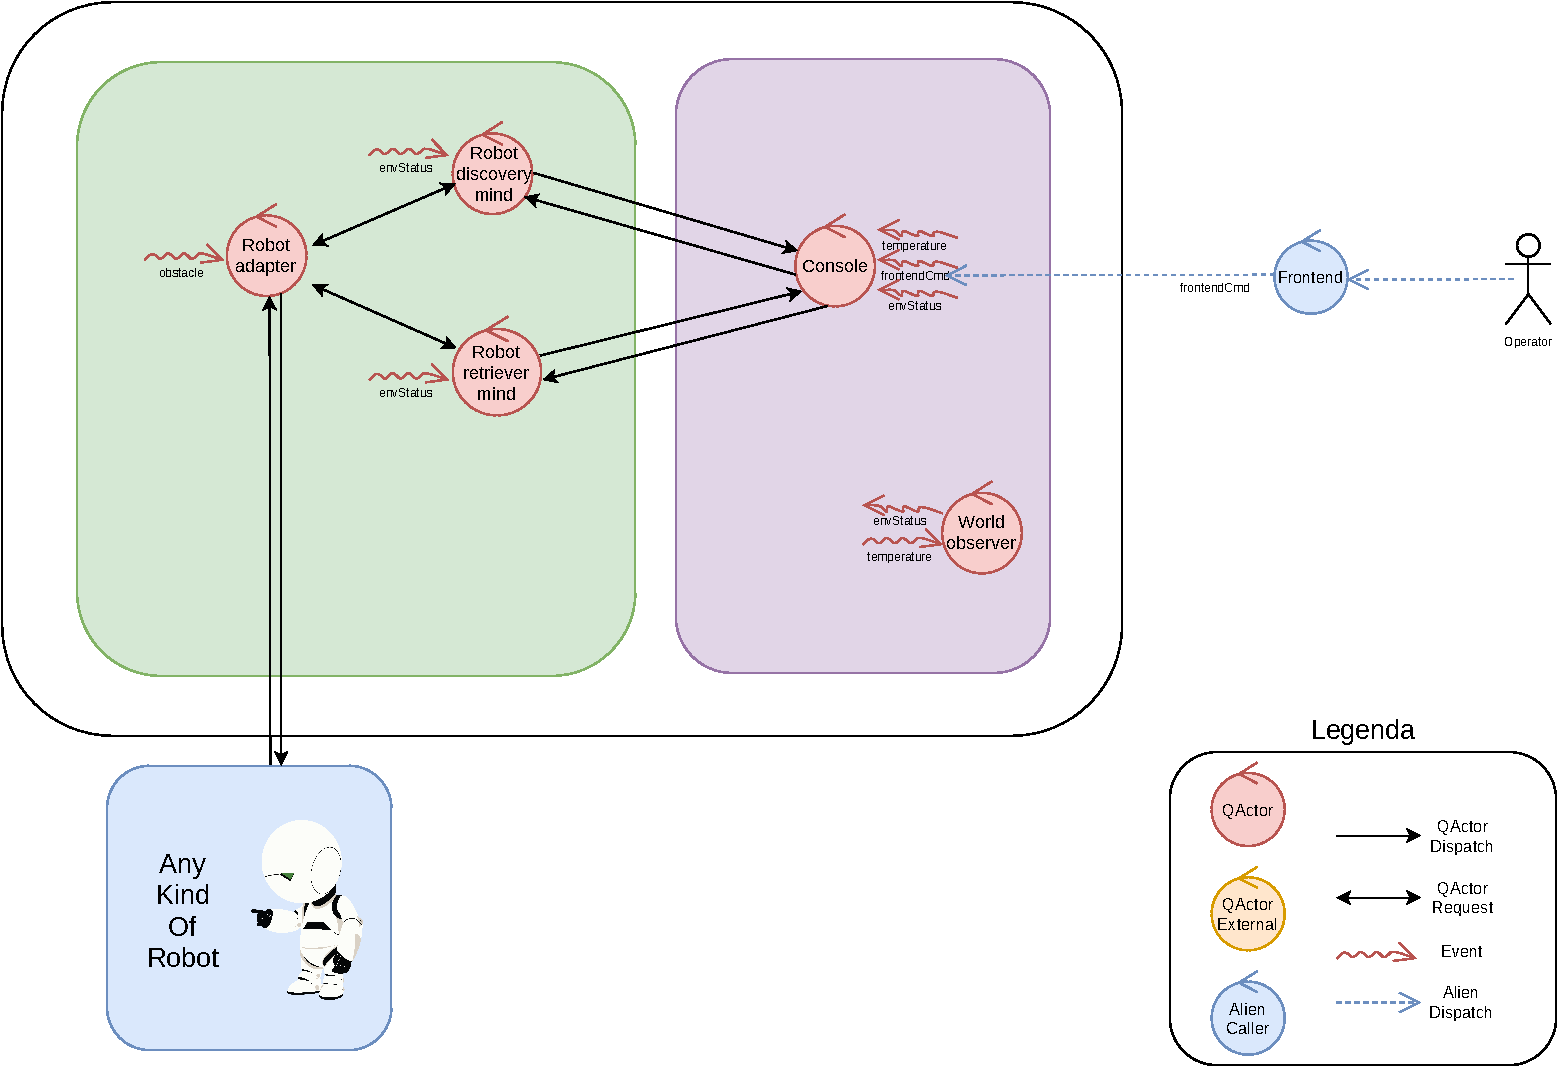
\includegraphics[width=0.85\textwidth]{res/analysis}%
  \caption{Grafico realizzato in draw.io che rappresenta lo stato del sistema in output all'analisi}%
  \label{fig:analysis}
\end{figure}

\newpage

\section{Progettazione}\labelsec{project}

Durante la fase di progettazione, sono state fatte le scelte necessarie a pianificare il lavoro per la realizzazione del sistema.

Per quanto riguarda le entità appartenenti al sistema, è risultato necessario scomporre il robot-adapter in entità più piccole, in modo da poter modularizzare meglio la logica implementativa:

\begin{description}
  \item[Robot Adapter] continua ad esistere come livello più basso, comportandosi come mero driver per le varie tipologie di robot.
  \item[Robot Advanced] si inserisce tra le due \textbf{Mind} e il \textbf{Robot Adapter} e introduce la possibilità di effettuare movimenti atomici sulla mappa, ora considerabile suddivisa in ``celle''.
  \item[One Cell Forward] viene adottato dalla codebase fornita dalla software house per lo spostamento tra le celle di una cella alla volte permettendo di mantenere lo stato consistente anche in presenza di ostacoli.
\end{description}

Le interazioni tra le entità sono a livello teorico delle request, in quanto ciascun comando impartito ha come risposta il nuovo stato;
purtroppo l'infrastruttura non metteva a disposizione delle vere request, di conseguenza si è optato per l'impiego di dispatch memorizzando manualmente il destinatario.

I messaggi e gli eventi precedentemente modellati sono i medesimi;
la componente di invio degli eventi è gestita tramite broker MQTT esterno (basato su Mosquitto e Docker).

Per quanto riguarda il componente alieno del frontend, esso è stato modellato come un server Express che interagisce tramite MQTT con il sistema, generando eventi.
L'utente interagisce con il server mediante un'interfaccia web in Angular servita dallo stesso, che diventa di fatto un client in esecuzione sul browser che interagisce tramite WebSocket con il server Express.

Di seguito, in~\Cref{fig:project} è possibile vedere una rappresentazione grafica del sistema per come è stato progettato e realizzato.

\begin{figure}[h]
  \centering%
  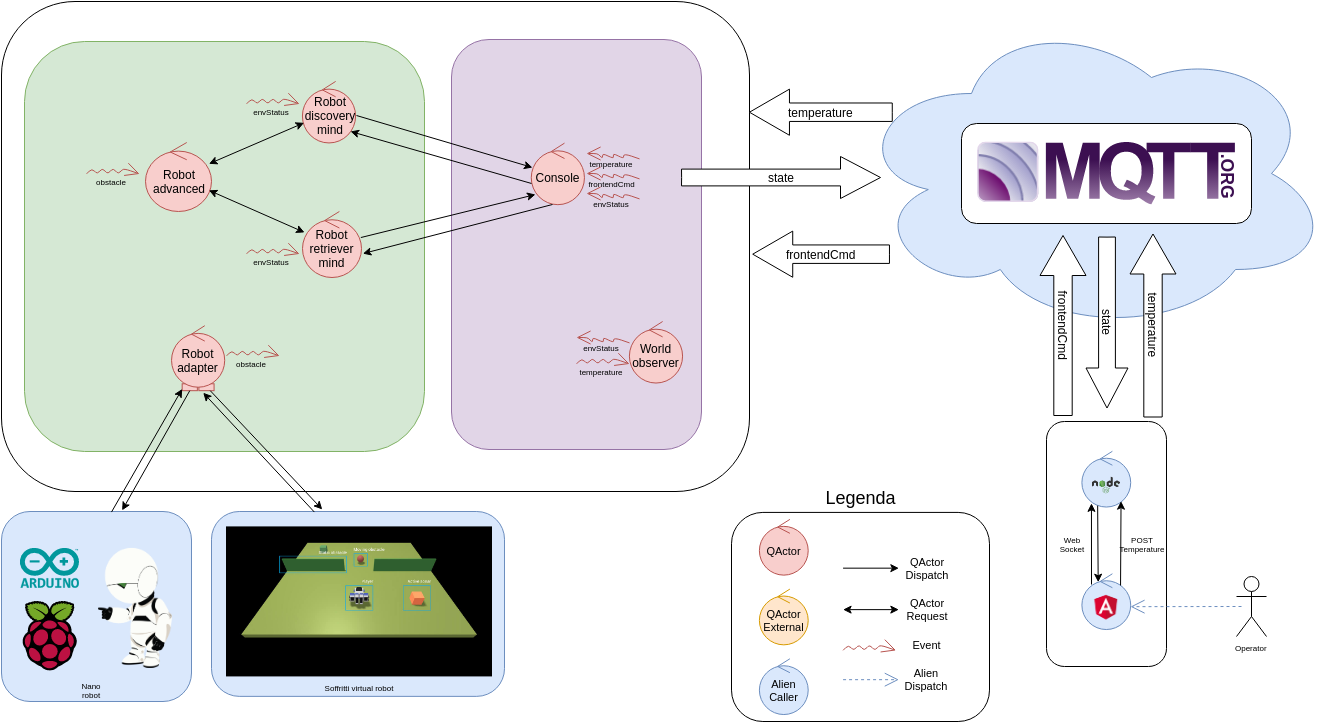
\includegraphics[width=0.85\textwidth]{res/project}%
  \caption{Grafico realizzato in draw.io che rappresenta lo stato del sistema in output alla fase di progettazione}%
  \label{fig:project}
\end{figure}

\end{document}
